\subsection{Software Design DAL Design}
På \autoref{fig:DAL-Klasse-7-17-18} herunder ses klassediagrammet over backend DAL, som benyttes til database access. 
Som det kan ses på diagrammet, indeholder DAL en database context, som benyttes til at forbinde backend applicationen til databasen. 
Derudover består DAL af fire overordnede funktioner, hvoraf de 3 tilhører en user story. 
Den sidste funktion benyttes når vi starter spillet, til at lave rumbeskrivelser.\\

\begin{figure}[H]
\centering
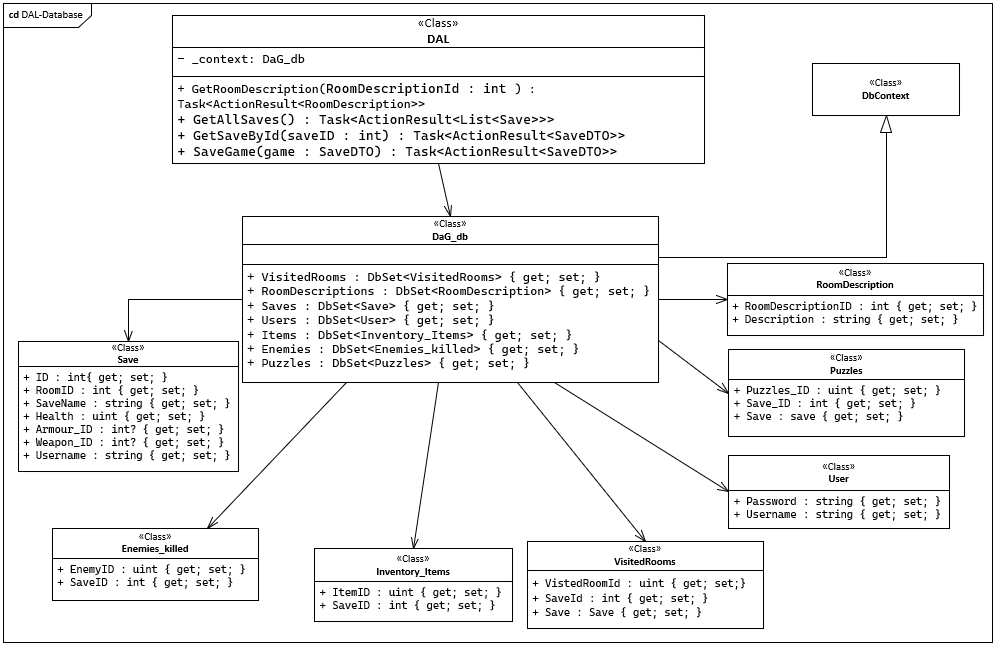
\includegraphics[width = \textwidth]{02-Body/Images/DAL-Database/DAL-DB-CD.PNG}
\caption{Samlet klasse diagram for User story 7, 17 og 18 med DAL db context og entitetsklasser.
For læseligheden er DAL klassen ikke forbundet til forskellige entitetsklasser selvom disse benyttes.}
\label{fig:DAL-Klasse-7-17-18}
\end{figure}

Følgende funktion som beskrives på \autoref{fig:DAL-Sekvens-RumBeskrivelser} benyttes når spil klienten startes, da beskrivelser af rum ikke ændre sig gennem spillets levetid, i den nuværende itteration.\\

\begin{figure}[H]
\centering
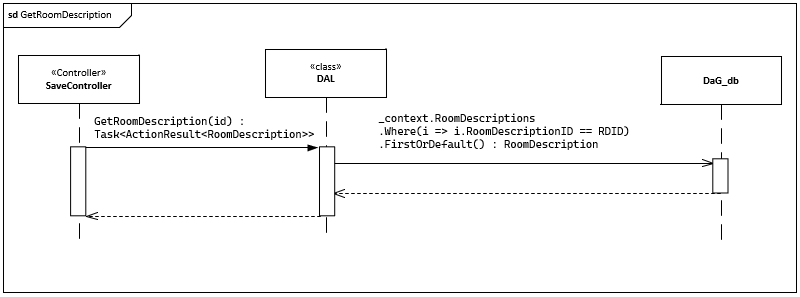
\includegraphics[width = \textwidth]{02-Body/Images/DAL-Database/RoomDescriptionSd.PNG}
\caption{Sekvensdiagram om læsning af en rumbeskrivelse}
\label{fig:DAL-Sekvens-RumBeskrivelser}
\end{figure}

Navn: GetRoomDescription \\
Parametre: int RoomDescriptionId \\
Returtype: Task\l ActionResult\l RoomDescription\g\g \\
Beskrivelse: Denne funktion finder og returnerer en beskrivelse for det valgte RoomDescriptionID. 
Dette kan også ses på sekvensdiagrammet på figur xxx herunder.


\subsubsection{User story funktioner}
De følgende 3 funktioner benyttes til udførelse af forskellige user stories.
Det drejer sig om:
\begin{itemize}
\item User story 7 – Save game
\item User story 17 – Load game list
\item User story 18 – Load game \\
\end{itemize}

Den første funktion SaveGame benyttes til at udføre user story 7.
Her skal der gemmes et spil.
Da vi har et krav om kun at holde 5 gemte spil pr. bruger, vælger vi at oprette 5 ”tomme” saves, når vi opretter brugeren.  
Når brugeren så ønsker at gemme et spil, skal vi ikke tilføje et nyt, men istedet overskrive et valgt gammelt save.
Dette kan også ses på sekvensdiagrammet på figur xxx.\\


\begin{figure}[H]
\centering
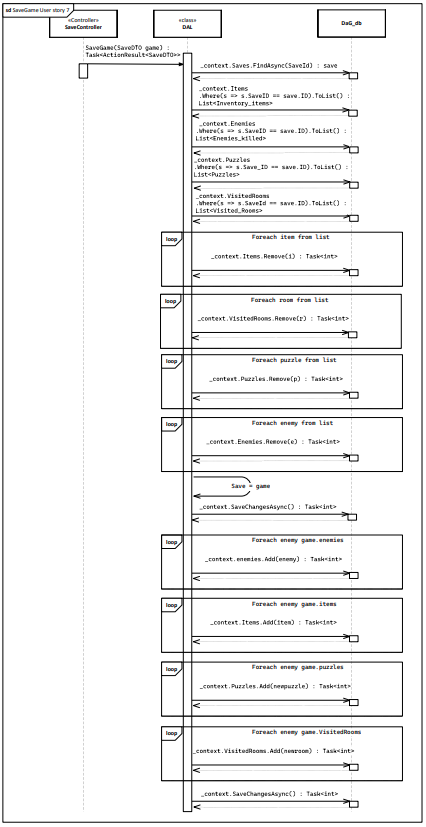
\includegraphics[width = 0.7\textwidth]{02-Body/Images/DAL-Database/SaveSd.PNG}
\caption{Sekvensdiagram for user story 7 save game som beskriver queries til databasen for at gemme et spil}
\label{fig:DAL-Sekvens-7}
\end{figure}


Navn: SaveGame\\
Parametre: SaveDTO\\
Returtype: Task\l ActionResult\l SaveDTO\g\g \\
Beskrivelse: Da der i vores frontend sørges for at en bruger blot kan have 5 saves, starter vi med at finde det save vi gerne vil overskrive. Det gamle save, samt tilhørende lister slettes, hvorefter det nye save gemmes og eventuelle nye lister til fx. items gemmes.\\

Den anden funktion GetAllSaves benyttes til at udføre user story 17.
Her skal der loades en liste af gemte spil, når brugeren ønsker at se sine gemte spil. Dette kan også ses på sekvensdiagrammet på \autoref{fig:DAL-Sekvens-17} .

\begin{figure}[H]
\centering
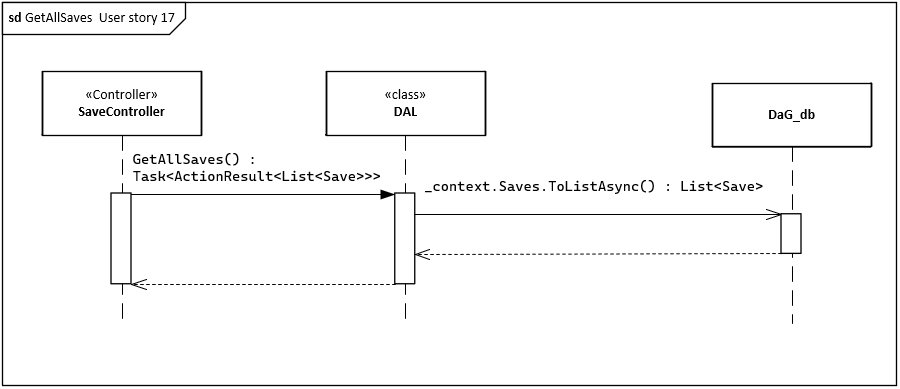
\includegraphics[width = \textwidth]{02-Body/Images/DAL-Database/GetSavesSd.PNG}
\caption{Sekvensdiagram for user story 17 GetAllSaves som beskriver queries til databasen for at hente alle saves}
\label{fig:DAL-Sekvens-17}
\end{figure}

Navn: GetAllSaves\\
Parametre: ingen\\
Returtype: Task\l ActionResult\l List\l Save\g\g\g \\
Beskrivelse: Her hentes all gemte saves i spillet.\\

Den tredje funktion GetById benyttes til at udfører user story 18.
Her skal der loades et gemt spil, som brugeren nu ønsker at spille. 
Dette kan også ses på sekvensdiagrammet på \autoref{fig:DAL-Sekvens-18}.\\

\begin{figure}[H]
\centering
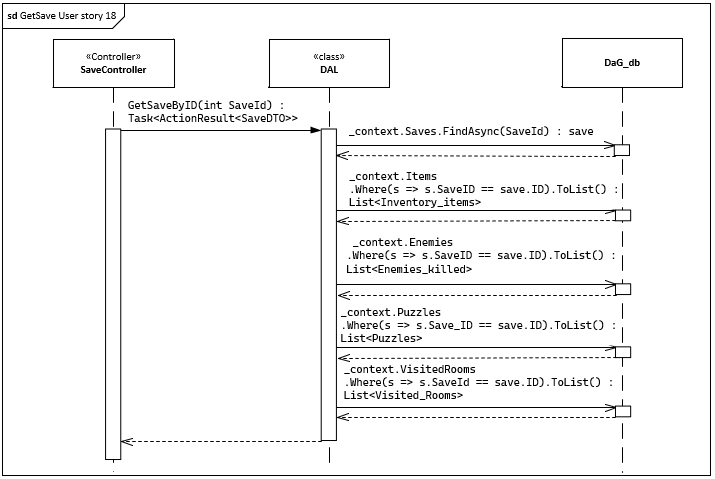
\includegraphics[width = \textwidth]{02-Body/Images/DAL-Database/GetSavesByIdSd.PNG}
\caption{Sekvensdiagram for user story 18 GetSaveById som beskriver queries til databasen for at hente et specifikt save og dens tilhørende information}
\label{fig:DAL-Sekvens-18}
\end{figure}

Navn: GetSaveById \\
Parametre: int saveID\\
Returtype: Task\l ActionResult\l SaveDTO\g\g\\
Beskrivelse: Denne funktion finder det save med det medsendte ID, samt tilhørende lister, indsætter værdier i et SaveDTO objekt, hvorefter det returneres.\\